\documentclass[twocolumn,10pt]{asme2ej}


%% The amssymb package provides various useful mathematical symbols
\usepackage{amssymb}
%% The amsthm package provides extended theorem environments
\usepackage{graphics,graphicx,amsbsy,amssymb}
\usepackage{epstopdf}
\usepackage{float}
\usepackage{import} 
\usepackage{color} 
\usepackage{tikz,pgfplots}
\usepackage[per-mode=symbol]{siunitx}
\usepackage{stfloats}
\usepackage{caption}
\usepackage{subcaption}

% Alter some LaTeX defaults for better treatment of figures:
    % See p.105 of "TeX Unbound" for suggested values.
    % See pp. 199-200 of Lamport's "LaTeX" book for details.
    %   General parameters, for ALL pages:
    \renewcommand{\topfraction}{0.9}	% max fraction of floats at top
    \renewcommand{\bottomfraction}{0.8}	% max fraction of floats at bottom
    %   Parameters for TEXT pages (not float pages):
    \setcounter{topnumber}{2}
    \setcounter{bottomnumber}{2}
    \setcounter{totalnumber}{4}     % 2 may work better
    \setcounter{dbltopnumber}{2}    % for 2-column pages
    \renewcommand{\dbltopfraction}{0.9}	% fit big float above 2-col. text
    \renewcommand{\textfraction}{0.07}	% allow minimal text w. figs
    %   Parameters for FLOAT pages (not text pages):
    \renewcommand{\floatpagefraction}{0.7}	% require fuller float pages
	% N.B.: floatpagefraction MUST be less than topfraction !!
    \renewcommand{\dblfloatpagefraction}{0.7}	% require fuller float pages

	% remember to use [htp] or [htpb] for placement


%% The lineno packages adds line numbers. Start line numbering with
%% \begin{linenumbers}, end it with \end{linenumbers}. Or switch it on
%% for the whole article with \linenumbers.
%% \usepackage{lineno}
% \journal{International Journal of Engineering Science}

\title{Characterization of a low relaxation time Oldroyd-B polymer solution using both numerical and experimental Continuous Ink Jet}

\author{Guillaume Ma\^itrejean
\affiliation{
    Laboratoire Rh\'eologie et Proc\'ed\'es\\
    Univ. Grenoble Alpes, LRP\\ F-38000 Grenoble France\\
    Email: guillaume.maitrejean@univ-grenoble-alpes.fr
}}

\author{Maxime Rosello
\affiliation{
    Laboratoire Rh\'eologie et Proc\'ed\'es\\
    Univ. Grenoble Alpes, LRP\\ F-38000 Grenoble France
}}
\author{Denis CD Roux
\affiliation{
    Laboratoire Rh\'eologie et Proc\'ed\'es\\
    Univ. Grenoble Alpes, LRP\\ F-38000 Grenoble France
}}
\author{Pascal Jay
\affiliation{
    Laboratoire Rh\'eologie et Proc\'ed\'es\\
    Univ. Grenoble Alpes, LRP\\ F-38000 Grenoble\\France
}}
\author{Jean Xing
\affiliation{
    Markem-Imaje Industries\\
    ZA de l'Armailler 9\\ rue Gaspard Monge\\
    BP 110 26501 Bourg-L\'es-Valence \\ France
}}
\author{Bruno Barbet
\affiliation{
    Markem-Imaje Industries\\
    ZA de l'Armailler 9\\ rue Gaspard Monge\\
    BP 110 26501 Bourg-L\'es-Valence \\ France
}}


\begin{document}
\maketitle 

\begin{abstract}
    The relaxation time of a weakly elastic polymer solution is measured by comparing numerical and experimental drop shapes. Computations use a viscoelastic Oldroyd-B model, the relaxation time of which is fitted using experimental results. This numerical approach is particularly convenient for weakly elastic solution physical parameters of which can not be measured by experimental rheometry.
\end{abstract}


%% \linenumbers

%% main text
\section{Introduction}
Capillary breakup phenomena have a wide range of applications from inkjet printing to DNA sampling. In micro jetting devices, polymer solutions often experience non Newtonian behaviour which greatly influence breakup dynamics. Drops generation from non Newtonian fluid jets breakup is a well known topic which has already been addressed both numerically and experimentally \cite{morrison2011inkjet,rodriguez2015experimental,mcilroy2013modelling}. Elastic and viscous effects are known to have a great influence on the breakup dynamics. More precisely, they are known to delay the onset of the jet breakup \cite{rayleigh1892xvi, gordon1973instability}. In the present work, the relaxation time of a weakly elastic ink used in industrial continuous inkjet printing (CIJ) devices is determinated. This ink is a low viscosity dilute polymer with high polydispersity. A first estimation of the elastic relaxation time is calculated using Zimm theory \cite{zimm1956dynamics}, and is found to be out of the measurement range of both extensional rheometry (ROJER \cite{keshavarz2015studying}) or microfluidic devices \cite{galindo2013microdevices}. As a result, an original approach is introduced to determine the relaxation time, relying on the comparison of capillary breakup shapes between numerical computations and experiments.

\section{Experimental setup}
The experimental device is similar to the one used for ROJER extensional rheometry measurements \cite{rodriguez2015experimental} (see figure 1). The flow is generated by a pump and the jet is created using a micro-nozzle. Then, it is strobed at a given frequency and synchronized with the drive frequency ($10 kHz < f_d < 100 kHz$) in order to display a static image ($1024\times778$ pixels with $1 px \approx 1 \mu m$ ). 

The visualization software is ImageXpert.

\begin{figure}[h]
    \centering
    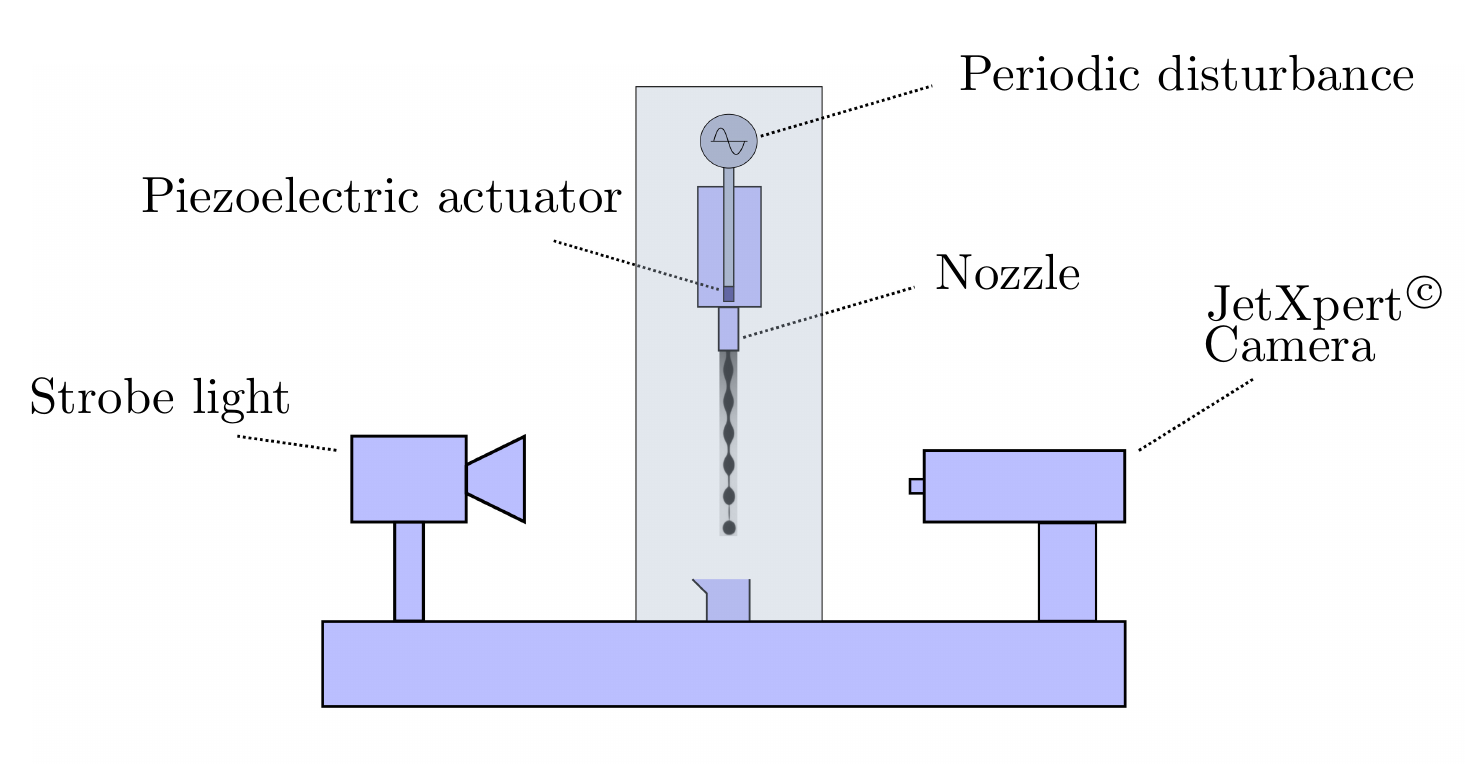
\includegraphics[width=8cm]{device.png}
    \caption{}
    \label{device}
\end{figure}

\begin{figure*}[t]
    \centering
    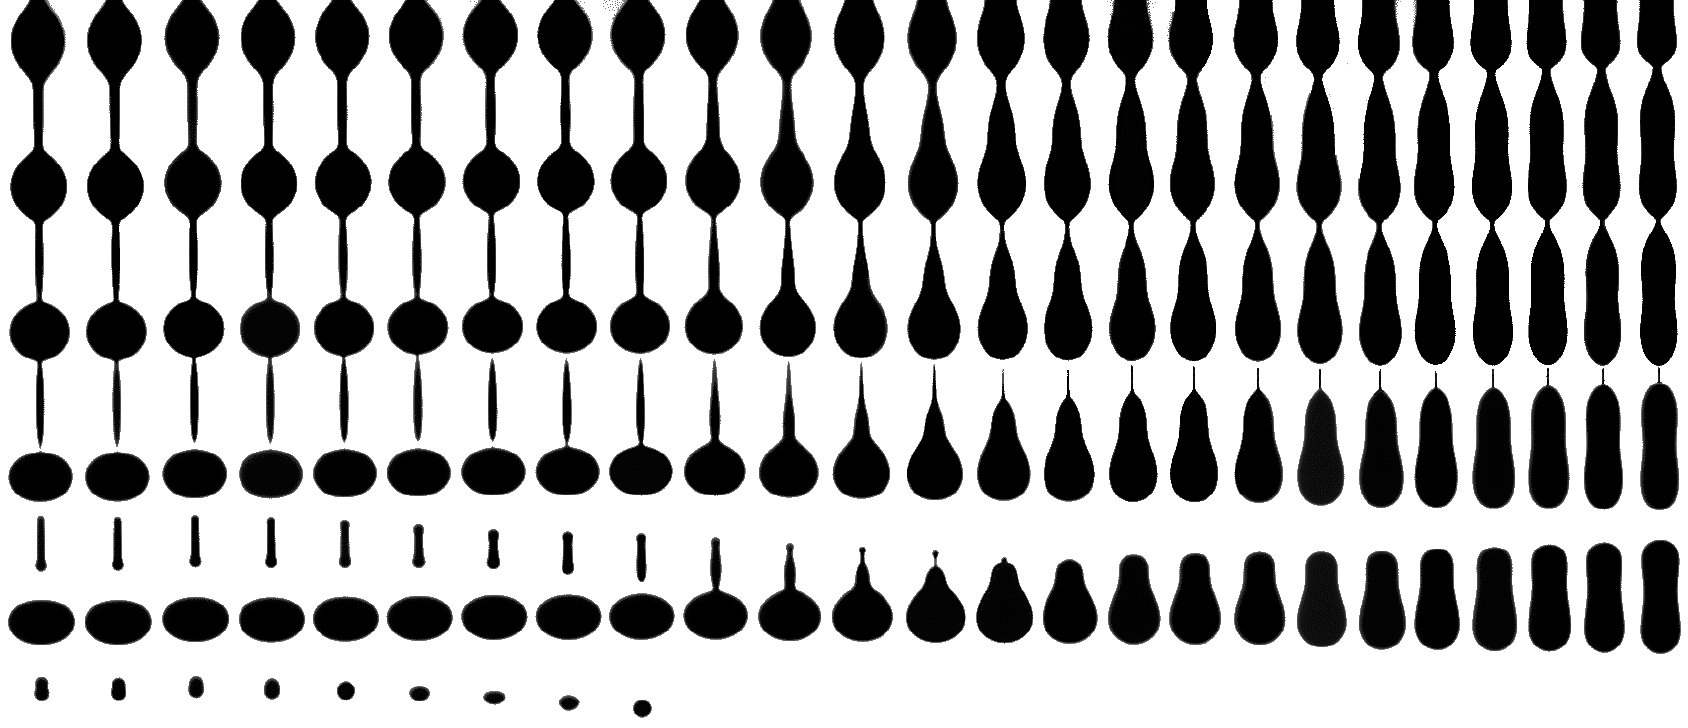
\includegraphics[width=0.8\textwidth]{Encre/expAll.png}
    \caption{Breakup shapes of the polymer solution for stimulation amplitudes ranging from 2V (left) to 62V (right).} 
    \label{fig:expAll}
\end{figure*}

Figure \ref{fig:expAll} depicts the morphology of the jets of the polymer solution addressed in the present paper and at the breakup distance from the nozzle. These jets have been generated  experimentally with the same device at stimulation amplitudes ranging from 2V to 62V and with a constant dimensionless wave number $x = 0.6$, where $x$ writes:
\begin{equation}\label{eq:waveNbr}
    x=2 \pi R_0 \frac{v}{f}
\end{equation}
with $R_0$ the radius of the unperturbed jet, $v$ the jet velocity and $f$ the stimulation frequency. Reynolds and Ohnesorgue numbers, respectively, are
\begin{equation}
    Re= \rho v R_0 / \eta_0 = 110
\end{equation} and 
   
\begin{equation}
    Oh=\eta_0/\sqrt{\rho R_0 \sigma} = 0.2
\end{equation}
are calculated for undisturbed jets. These numbers are constant for every disturbance amplitudes.

For high stimulation amplitude, We observe threads linking the first droplets to the unbroken jet which is typical of breakup of weakly elastic polymer strain hardening solutions \cite{christanti2002effect}.

Figure \ref{fig:LbInk} shows the breakup length as a function of the disturbance amplitude, i.e. as a function of the tension applied to the piezoelectric actuator. The so called breakup length, also called "intact length", has been widely studied both in linear and non-linear regime, see \cite{eggers2008physics} and therein references, and is directly linked to the nozzle outlet velocity disturbance \cite{pimbley1977satellite} and \cite{rosello2018influence} and, as expected the breakup length decreases with the disturbance amplitude.

\begin{figure}[H]
    \centering
    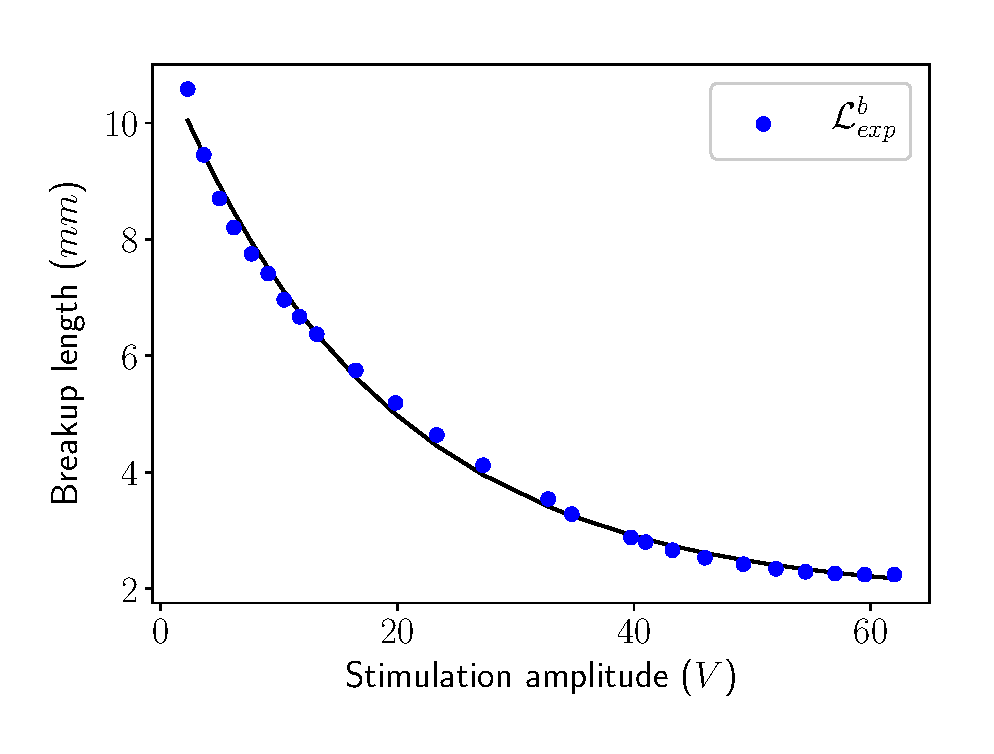
\includegraphics[width=8.5cm]{LbInk.eps}
    \caption{}
    \label{fig:LbInk}
\end{figure}



\subsection{Rheological characterization}\label{sec:rheo}

The density $\rho = 873 kg.m^{−3}$ and the surface tension $\sigma = 22.8 mN.m^{-1}$ of the fluid have been carefully measured using an Lovis 2000MME device from Anton Paar and a MPT2 from Lauda, respectively. 

The shear viscosity is measured using both ARG-2 from TA-Instruments for low shear rates ($\dot{\gamma} < 1000 s^{−1}$ ) and m-VROC from RheoSense for high shear rates ($1000 s^{−1}<\dot{\gamma} < 10^6 s^{−1}$). As we can see on figure \ref{beahaviorLaw}, the viscosity shows a slight shear-thinning behavior around $10^6s^{-1}$, and considering the incertitude of measure, the fluid viscosity is assumed constant over the full range of shear rate.

\begin{figure}[H]
    \centering
    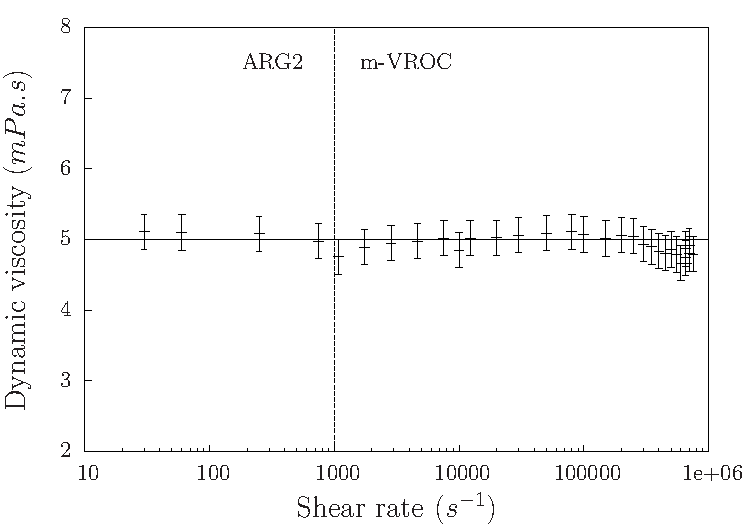
\includegraphics[width=8cm]{./9651visco.eps}
    \caption{Dynamic viscosity of the present polymer solution as a function of the shear rate.}
    \label{beahaviorLaw}
\end{figure}

As stated in the previous section, the polymer solution presents a weakly elastic solution. Zimm theory can thus be used to describe polymer relaxation dynamics considering hydrodynamic interactions between chains and solvent. This theory is particularly accurate for dilute polymer solutions and enables the calculation of a relaxation time $\tau_Z$ , such as :
\begin{equation}
    \tau_Z = \frac{\eta_s [\eta] M}{RT} = 0.4 \mu s
    \label{zimm} 
\end{equation}
with $\eta_s$ the solvent viscosity in $Pa.s$, $[\eta]$ the intrinsic viscosity in $m^3.kg^{−1}$ , $M_w$ the
polymer molecular mass $kg.mol^{−1}$ , $R$ universal gas constant and $T$ the temperature in $K$.

Let us consider the capillary time scale $\tau_c$ , given by :
\begin{equation}
    \tau_C= \sqrt{\rho R_0^3 / \sigma}
\end{equation}
with unperturbed $R_0$ the jet radius. 

In the present work, the polymer relaxation time predicted by Zimm theory is very small compared with the capillary time scale, so that elasticity should have a negligible influence on the breakup dynamics for small to moderate stimulation amplitude. 

However, this low relaxation $\tau_Z<<\tau_C$ time prevent us from using the jetting device as a ROJER \cite{keshavarz2015studying} in order to measure the relaxation time. 

To the knowledge of the authors, no experimental device can capture such a short relaxation time and we follow another route in section \ref{numericalDetermination} by comparing numerical simulation to experimental results in order to determine it.

\section{Validation of the numerical model}
The computation is performed using OpenFoam and more specifically with its multiphase solver interFoam \cite{deshpande2012evaluating}. In order to evaluate the ability of the solver to numerically model the jetting of a non-Newtonian fluid, it is first assessed on the well-known capillary instability growth of a Newtonian fluid and eventually jetting of Newtonian fluid is considered.

\subsection{Simulation of the capillary instability growth}
We first assess the performance of the interFoam solver by simulating the growth of a perturbation at the surface of a column of Newtonian liquid. The results can then be compared to the linear theory first derived by Rayleigh \cite{rayleigh1892xvi} and then enhanced by \cite{chandrasekhar2013hydrodynamic}, which provides well-known test case \cite{delteil2011numerical,cervone2010simulation}.
The analytical dispersion equation from \cite{chandrasekhar2013hydrodynamic} writes:
\begin{equation}
    \gamma \tau_c = \sqrt{\frac{1}{2}(x^{2}-x^{4}) + \frac{9}{4}Oh^{2}x^{4}}-\frac{3}{2}Oh x^{2},
    \label{eq:growthRateAnalytical}
\end{equation}
with $\gamma$ the growth rate, $\displaystyle \tau_c = \sqrt{\frac{\rho_f R_0^3}{\sigma}}$ the capillary time, $x$ the dimensionless wave number and $Oh$ the Ohnesorgue number
\begin{equation}
    Oh=\frac{\eta}{\sqrt{\rho \sigma R_0}}.
    \label{eq:Oh2}
\end{equation} 

Simulation of the capillary instability growth consists in an axisymmetric flow within a rectangular domain of width $\lambda$ and height $h$, and composed of a liquid of radius $R_0$ and a gaz. At $t = 0s$ the liquid is at rest and a small perturbation of wavelength $\lambda$ and amplitude $\delta$ is applied to its surface. 
Domain is meshed with square elements of side $\Delta_x$ and simulation is found to converge with $\Delta_x< 7\,10^{-5}m$. Parameters of the simulation are summed up Table \ref{tab:parametersPinch} and Fig \ref{fig:capillaryGrowth} shows numerical results at different time $t \in [0s,2s]$.

\begin{table}
    \begin{center}
        \begin{tabular}{lr}
            \hline
            $\rho_{l} (kg.m^{-3})$ & $1000$\\
            $\rho_{g} (kg.m^{-3})$ & $1$\\
            $\nu_{l} (Pa.s)$ & $10^{-3}$\\
            $\nu_{g} (Pa.s)$ & $10^{-6}$\\
            $h(m)$ & $28\, 10^{-4}$\\
            $\lambda (m)$ & $64\, 10^{-4}$\\
            $R_0(m)$ & $7.07\, 10^{-4}$\\
            $\delta (m)$ & $1.6\, 10^{-5}$\\
            $Oh$ & $0.2$\\
            $\tau_{c}(s)$ & $0.1$  \\   
            $\Delta_x(m)$ & $7\,10^{-5}$ \\      
            \hline
        \end{tabular}
    \end{center}
    
    \caption{\label{tab:parametersPinch}Parameters of capillary instability simulations.}
\end{table}

\begin{figure*}[t]
    \centering
    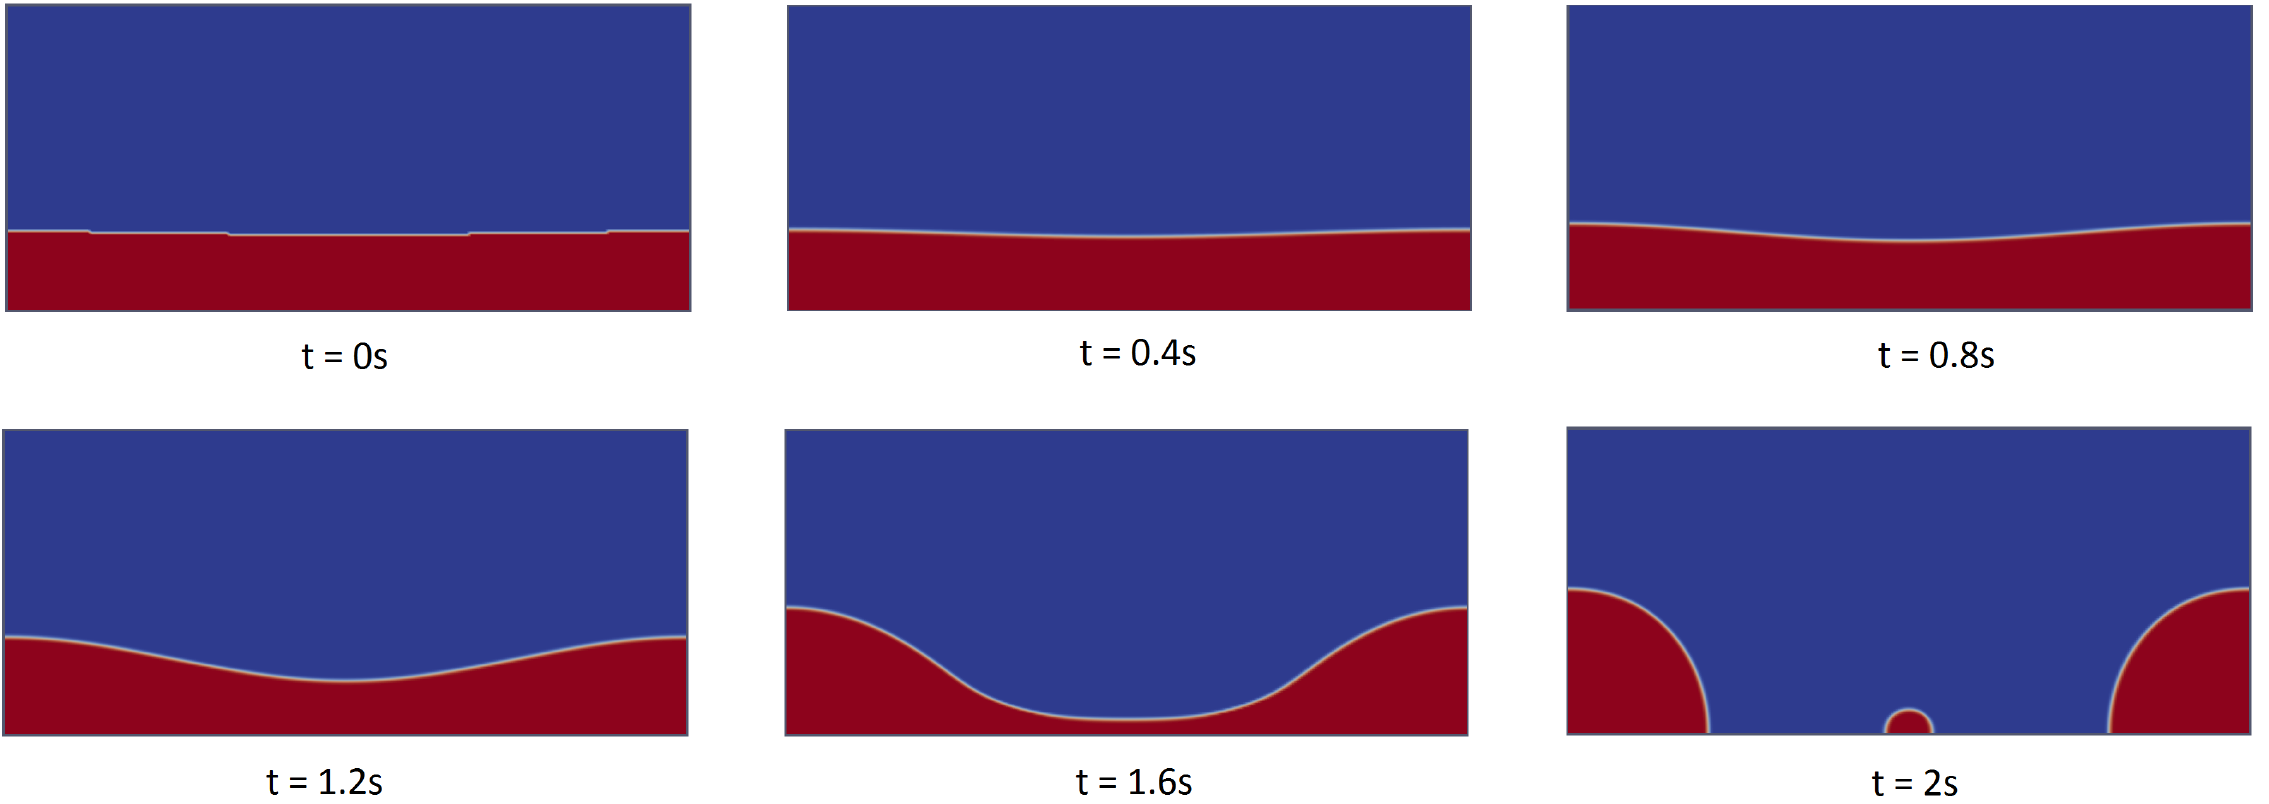
\includegraphics[width=\textwidth]{pinch.png}
    \caption{Evolution of the capillary instability (liquid in red and gaz in blue)} 
    \label{fig:capillaryGrowth}
\end{figure*}

Comparison of theoretical growth rate from Eq. \ref{eq:growthRateAnalytical} with numerical results Fig. \ref{fig:growthrate} shows good agreement as analytical solution is based on linearized approach whereas interFoam solves full Navier-Stokes equation.

\begin{figure}[h]
    \centering
    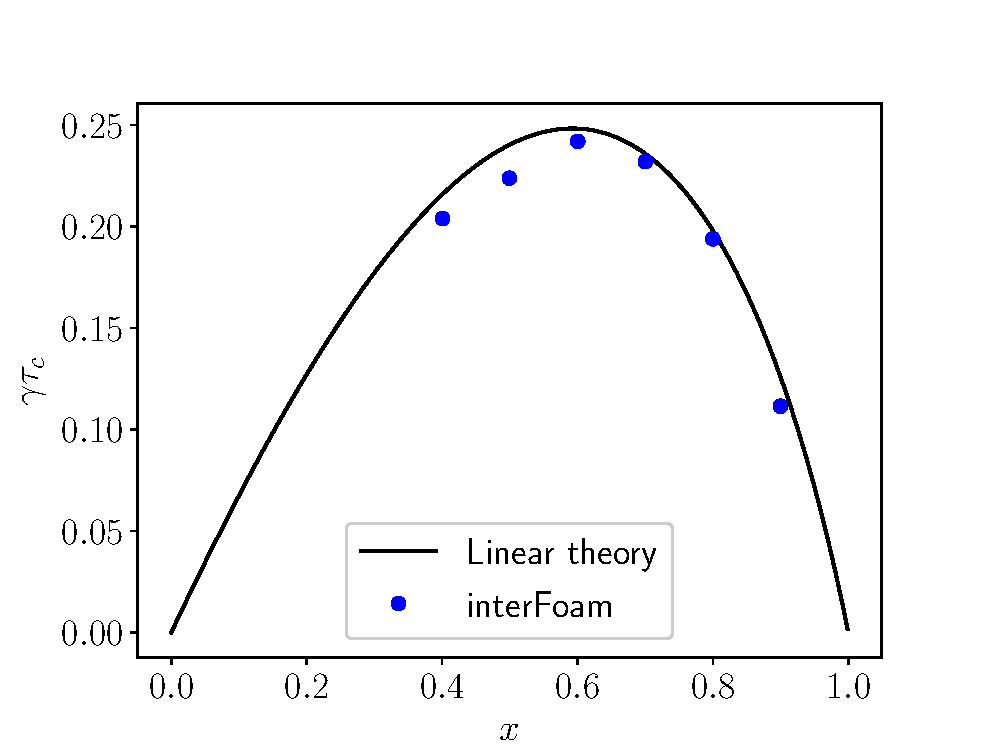
\includegraphics[width=8cm]{dispersion.eps}
    \caption{Growth rate $\gamma \tau_c$ as a function of of the dimensionless wave number $x$}
    \label{fig:growthrate}
\end{figure}

\subsection{Numerical simulation of Newtonian CIJ}\label{sec:glycerol}
In order to fine tune the numerical model for CIJ cases, jetting of a Newtonian solution of water and glycerol is addressed. The density, viscosity and surface tension of the solution has been carefully measured using, respectively, an Anton Paar DMA4500, an Anton Paar Lovis 2000MME and a Lauda MPT-2. Table \ref{tab:parametersGlycerol} sums up the physical properties of the solution used in the numerical simulation.

\begin{table}
    \begin{center}
        \begin{tabular}{lr}
            \hline
            $\rho_{l} (kg.m^{-3})$ & $1128.88$\\
            $\nu_{l} (mPa.s)$ & $6.4$\\
            $\sigma (mN.m^{-1})$ & $69.16$\\
            \hline
        \end{tabular}
    \end{center}
    
    \caption{\label{tab:parametersGlycerol} Physical parameters of glycerol + water solution.}
\end{table}

Figure \ref{fig:glycerolCIJExp}(a-i) shows experimental jets for different stimulation amplitude (given in Volts). 

\begin{figure*}[t]
    \centering
    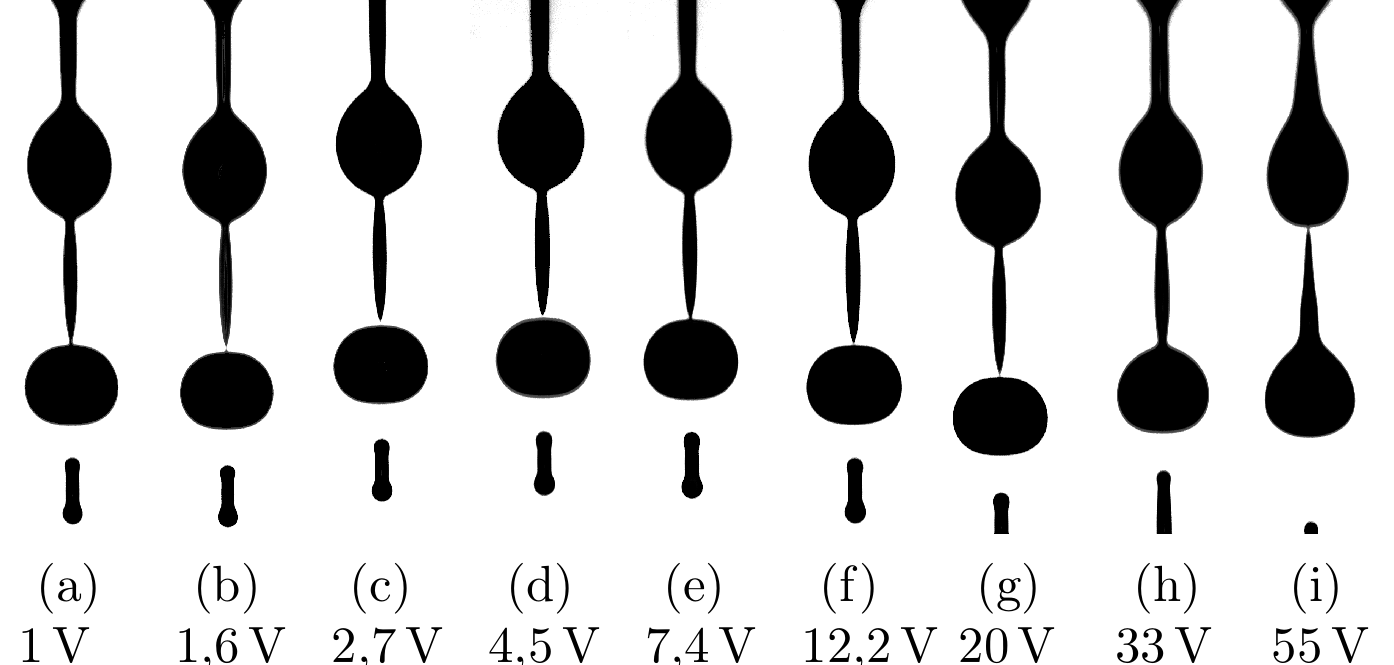
\includegraphics[width=10cm]{Glycerol/gouttes_exp.png}
    \caption{Experimental jets for different stimulation amplitude (in Volts) located a the breakup length.}
    \label{fig:glycerolCIJExp}
\end{figure*}

The numerical model of the CIJ device takes advantage of the axisymmetry of the problem the upper part of the numerical domain, which is thus 2-dimensional and includes fluid tank and nozzle, is depicted Fig. \ref{fig:meshGlycerol}. 

At $t=0s$, both tank and nozzle are filled with fluid and the rest of the domain is filled with air. In order to jet the fluid, a pressure Dirichlet boundary condition is applied on the inlet of the domain (left side of the tank) such as:
\begin{equation} \label{eq:plim}
    P=P_{tank}+P_{stim}\cos(2\pi f t)
\end{equation}
where $P_{tank}$ and $P_{stim}$ are related, respectively, to the absolute steady pressure in the fluid tank, driving the jetting velocity of the fluid, and the amplitude of stimulation.
\begin{figure}[H]
    \centering    
    \begin{tikzpicture}
        \node[anchor=south west,inner sep=0] (0,0) {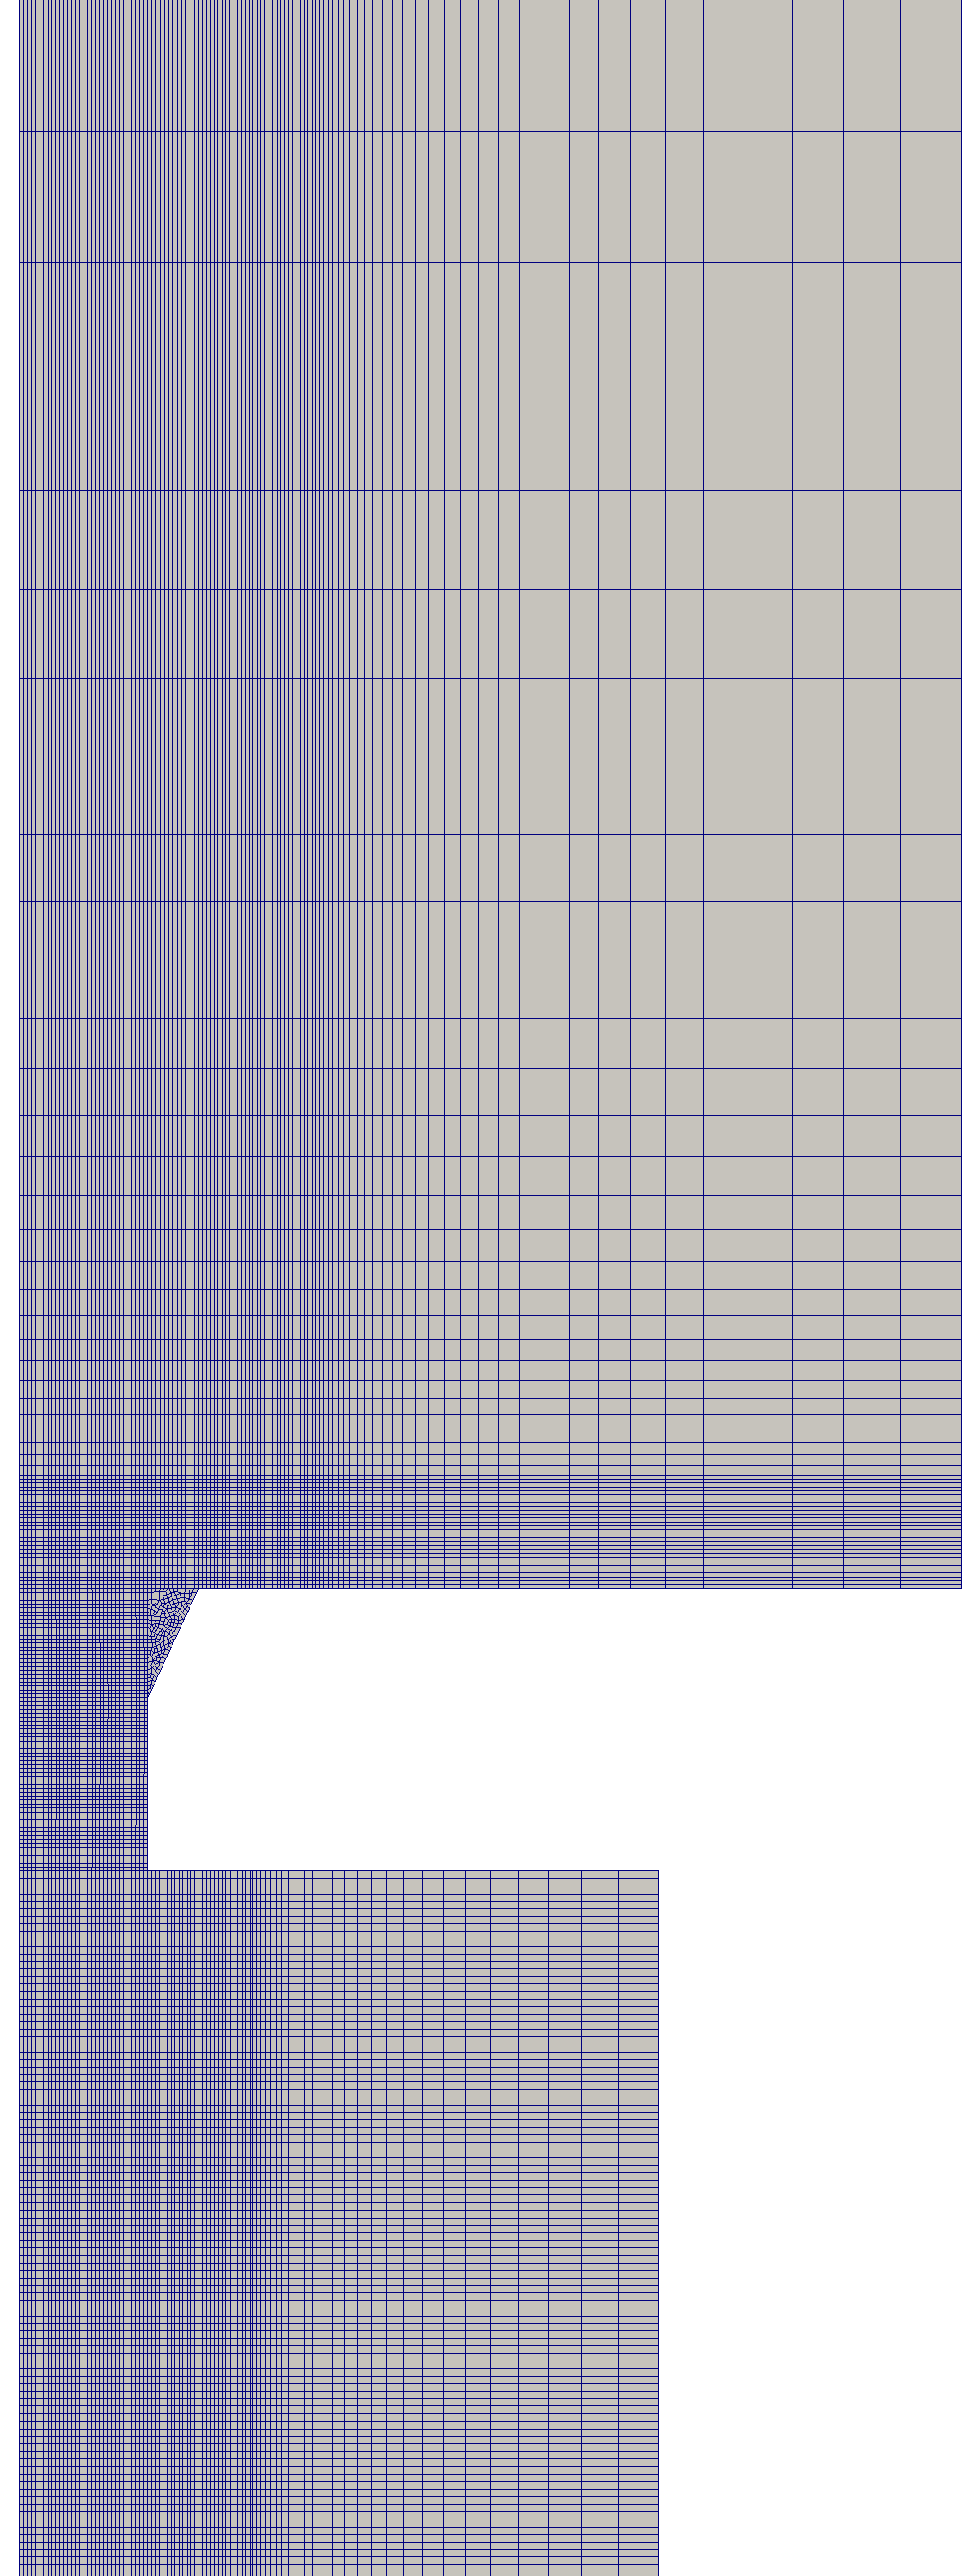
\includegraphics[width=3cm,angle=90]{maillage.png}};
        
        \draw[dashed] (0,3) -- (0,3.3);       
        \draw[dashed] (4.8,3) -- (4.8,3.3);
        \draw[dashed] (5.75,2.05) -- (5.75,3.3);
        \draw[dashed] (7.9,2.05) -- (7.9,3.3);
        
        \draw (2.5,3.5) node {Fluid Tank};
        \draw (5.3,3.5) node {Nozzle};
        \draw (6.9,3.5) node {Air};
        
        \end{tikzpicture}
    \caption{Converged mesh of the tank, nozzle and nozzle outlet of the axisymmetric numerical model.} 
    \label{fig:meshGlycerol}
\end{figure}

To accurately determine $P_{tank}$, both the mass flow and the dimensionless wave number $x$ are experimentally measured and compared to numerical results by try and error process.In the present case the $P_{tank}$ has been found $P_{tank}=4140 \, mbar$. 


$P_{stim}$ is directly related to the tension applied to the piezoelectric actuator and there is no direct relation between the amplitude of stimulation in Volt and the one in Pascal. In order to determine the pressure exerted on the fluid by the piezoelectric device, i.e. $P_{stim}$, as a function of the tension applied $T_{stim}$, we must compare experimental and numerical breakup jets. One way to do so lies in comparing droplet shapes, but in this present case and due to the hight tension surface exhibited by the glycerol solution, the droplets created looks very similar (see Fig. \ref{fig:glycerolCIJExp}) and one can not use this criterion to discriminate the jets. We then use the breakup lengths of the jets, respectively, $\mathcal{L}_{exp}^b$ and $\mathcal{L}_{num}^b$, to assess the relation between $P_{stim}$ and $T_{stim}$. 

\begin{figure}[h]
    \centering
    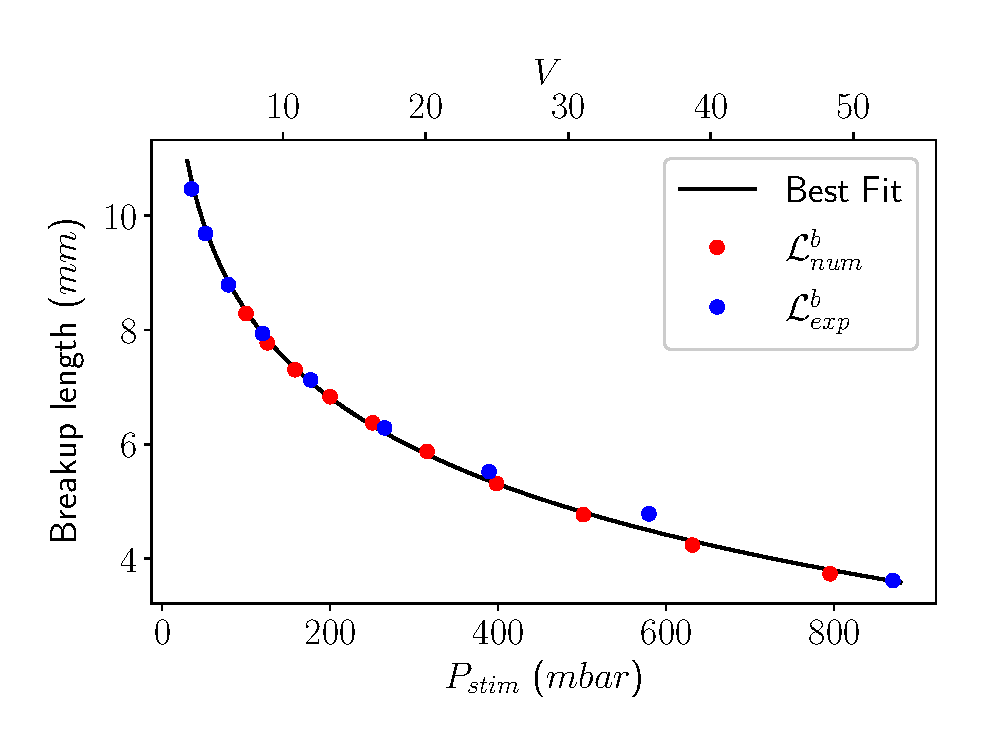
\includegraphics[width=8.5cm]{LbGlycerol.eps}
    \caption{Numerical and Experimental breakup lengths for glycerol solution.}
    \label{fig:LbGlycerol}
\end{figure}

Figure \ref{fig:LbGlycerol} shows both $\mathcal{L}_{exp}^b$ and $\mathcal{L}_{num}^b$ and an excellent agreement can be found between $P_{stim}$ and $T_{stim}$:
\begin{equation}
    P_{stim} = 36.4 \, T_{stim}^{0.792}
\end{equation}


\begin{figure}[h]
    \centering
    \begin{subfigure}{2.7cm}
        \centering
        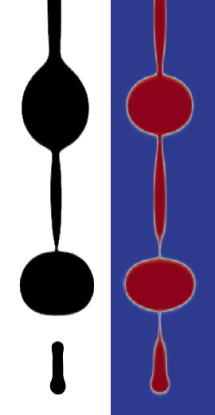
\includegraphics[width=2.5cm]{Glycerol/num_exp_053mbar_1.png}
        % \captionsetup{font={scriptsize,it}}
        \caption{1.6$V$ - 53$mbar$}
    \end{subfigure}
    \hfill
    \begin{subfigure}{2.7cm}
        \centering
        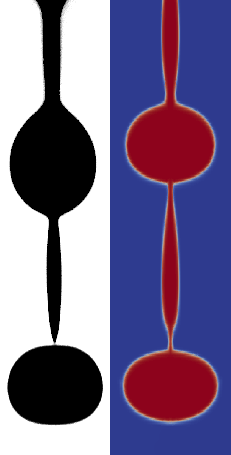
\includegraphics[width=2.5cm]{Glycerol/num_exp_264mbar.png}
        \caption{12.2$V$ - 264$mbar$}
        % \label{fig:three sin x}
    \end{subfigure}
    \hfill
    \begin{subfigure}{2.7cm}
        \centering
        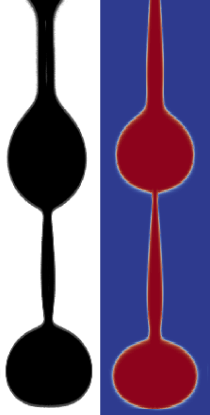
\includegraphics[width=2.5cm]{Glycerol/num_exp_580mbar_1.png}
        \caption{33$V$ - 580$mbar$}
        % \label{fig:five over x}
    \end{subfigure}
       \caption{Comparison between experimental (black and white) and numerical (colour) droplet shapes for different amplitudes of stimulation}
       \label{fig:glycerolDrop}
\end{figure}
It is worth noting that the numerical breakup length can strongly impacted by the mesh as $\mathcal{L}_{num}^b$ relates to the length where fluid thread thickness tends towards zero. However the high surface tension exhibited by the glycerol solution prevent $\mathcal{L}_{num}^b$ to diverge from $\mathcal{L}_{exp}^b$ and excellent agreement is found between them both. 

Droplet shapes depicted \ref{fig:glycerolDrop}(a-c) shows excellent agreement between numerical and experimental results and satellites dynamic is also captured by the numerical model from low ($1.6V$) to high amplitude stimulations ($33V$).


\section{Numerical determination of the relaxation time} \label{numericalDetermination}
The computation is performed using the previously finetuned interFoam solver (see section \ref{sec:glycerol}) and the same 2D-axisymmetric geometry. 

Neither shear thinning nor strain thickening behavior is expected, thus the Oldroyd-B viscoelastic model \cite{oldroyd1950formulation} is assumed to accurately describe the viscoelastic behavior of the present work. 

The solvent and polymer contribution to viscosity, respectively $\eta_s$ and $\eta_p$ have been carefully measured and the influence of the relaxation time $\tau_e$ onto the breakup shape is investigated. Giving the value $\tau_z= 0.4 \mu s$ found in section  \ref{sec:rheo}, $\tau_e$ from $0.5 \mu s$ to $1 \mu s$ will be tested. 

The relaxation time has an influence on the average jet velocity $v$ : the more elastic the fluid, the slower the jet. Thus, the instability wave number $x$ (see \ref{eq:waveNbr}) increases when $\tau_e$ increases. Consequently $P_{tank}$ depends on $\tau_e$ and has been determined by ensuring a constant dimensionless wave number $x=0.6$ for unperturbed viscoelastic jets (i.e. setting $P_{stim}=0$ in eq. \ref{eq:plim}). Figure \ref{fig:dP} shows the linear relation found between $P_{tank}$ and the fluid relaxation time in order to get $x=0.6$.

\begin{figure}[H]
    \centering
    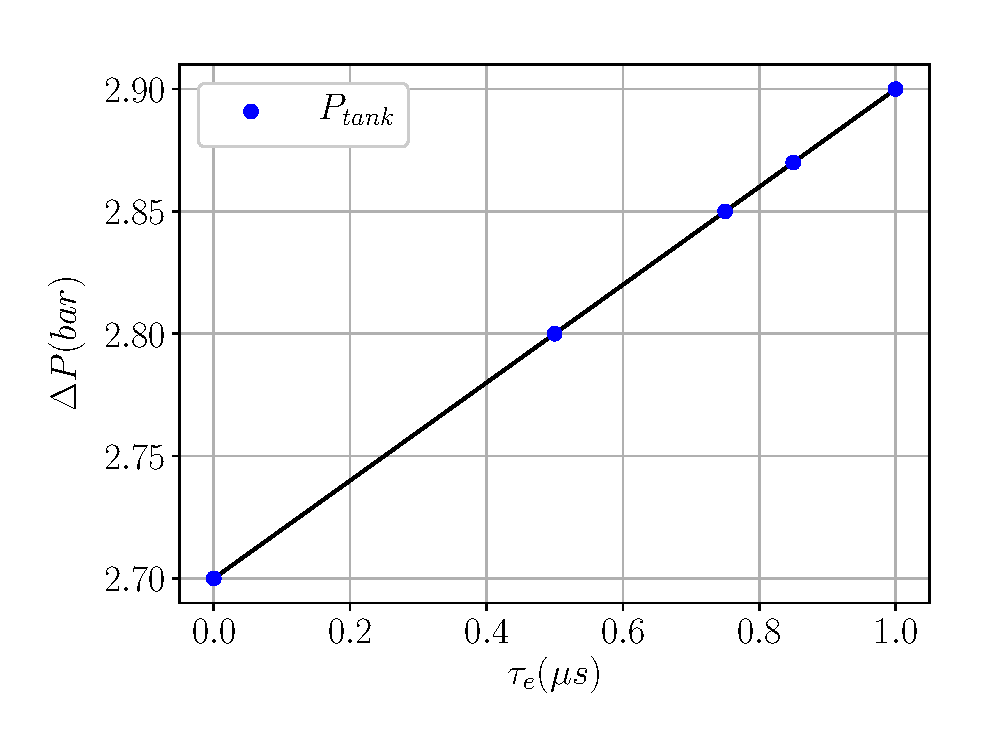
\includegraphics[width=8.5cm]{dP.eps}
    \caption{$P_{tank}$ as function of $tau_e$.}
    \label{fig:dP}
\end{figure}

It is worth pointing out that over the studied range of relaxation times, the jet does not exhibit die-swell effect at the nozzle exit : the dependence of $R_0$ with $\tau_e$ is then assumed negligible, and, consequently, $P_{tank}$ only influences the value of the jet averaged velocity $v$. Moreover Figure \ref{fig:vProfiles} presents the axial velocity profile at the nozzle outlet obtained for $\tau_e = 0\mu s$ (Newtonian), $\tau_e = 0.5\mu s$ and $\tau_e = 1\mu s$ for a jet without disturbance. It seems that within the studied relaxation time range, elasticity has a small influence onto velocity profiles.

\begin{figure}[H]
    \centering
    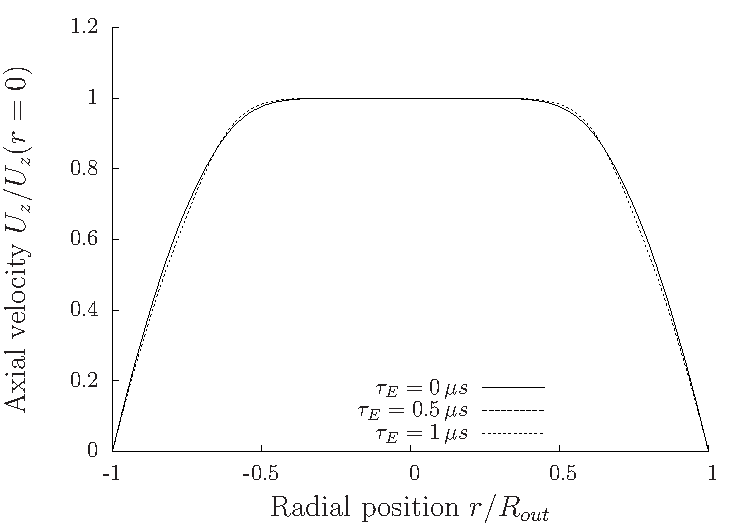
\includegraphics[width=8.5cm]{vProfiles.eps}
    \caption{Computational axial velocity profiles at the nozzle exit for the Newtonian jet ($\tau_e = 0\mu s$) and Oldroyd-B fluids ($\tau_e = 0.5\mu s$ and $\tau_e = 1\mu s$).}
    \label{fig:vProfiles}
\end{figure}

From now on, a disturbance is applied to the jet using the pressure boundary condition (see eq. \ref{eq:plim}). In order to compare the numerical results to the experimental ones, one must find the relation between $P_{stim}$ and $V_{stim}$, which denote, respectively, the numerical and experimental disturbance amplitudes. In section \ref{sec:glycerol} the correlation has been found based on the breakup length. 

However, as previously stated, the breakup length criterion is not fully appropriate for low to moderate surface tension fluids as it may depends on numerical parameters. The results are thus compared using both the breakup length and the breakup shapes which are highly influenced by the disturbance amplitude as pictured Figures \ref{fig:expAll} and \ref{fig:LbInk}. 

For each numerical fluid, i.e. Newtonian
\begin{table}
    \begin{center}
        \begin{tabular}{l|cc}
            Fluids & $\mathcal{L}^{0.3}_b\,(mm)$ &$\mathcal{L}^{0.5}_b\,(mm)$\\
            \hline
            Experimental  &  & \\
            Newtonian & 2.85 & 2.54\\ 
            $\tau_e = 0.5\mu s$ & 3.3 & 2.25\\ 
            $\tau_e = 0.75\mu s$ & 3.95 & 2.85\\ 
            $\tau_e = 0.85\mu s$ & 4.45 & 4.25\\ 
            $\tau_e = 1\mu s$ & 5.5 & $> 6.5$\\ 
            \hline
        \end{tabular}
    \end{center}
    
    \caption{\label{tab:lbInk}.Breakup lengths $\mathcal{L}^{0.3}_b$ and $\mathcal{L}^{0.5}_b$ of the numerical and experimental fluids. }
\end{table}

\bibliographystyle{asmems4}
\bibliography{biblio}
\end{document}
